\section{NLP Engine methodology}\label{sec:methodology}
In general, our design consists of the following two approaches (which we discuss in more detail in this section): \textit{detection} and \textit{comparison}. While \textit{detection} has symbols as basic processing unit, \textit{comparison} has sub-articles as basic processing unit. \textit{Detection} represents the capability to detect \textit{variables} in a text file, i.e., the RA. For this purpose, \textit{Amazon Comprehend} constitutes the enabling technology of the \textit{detection} approach, since it is a service that uses NLP techniques to extract insights about the content of text documents by recognizing  the  entities,  key  phrases,  language,  sentiments,  and  other  common  elements  in  a  text~\cite{AWS2021}.

\textit{Comparison} represents the capability to find \textit{similarities} and differences between the sub-articles present in the RA concerning the sub-articles present in the GSMA standard template. In this regard, \textit{text similarity}~\cite{Deza2009} constitutes the enabling technology of the \textit{comparison} approach, since it is a resource commonly used for pattern classification, clustering, and information retrieval problems~\cite{7429408}. We employ \textit{Jaccard's similarity} which is defined as the size of the intersection divided by the size of the union of two sets~\cite{Gupta2018}. As a result of the \textit{comparison}, it is determined that while an almost total coincidence between texts at the sub-article level represents a \textit{standard clause}, an almost null coincidence between texts (or simply the non-existence of a sub-article of the GSMA standard template in the RA) represents a \textit{customized text}. Thus, the intermediate case is represented by the \textit{variation} in which there is a high coincidence between sub-articles, and the existing differences are given by the presence of \textit{variables} such as the commercial names of MNOs and the start date of the RA. The next section integrates tools, NLP techniques, and text processing techniques as part of the designed methodology.

\subsection{Designed Methodology}
The flow chart in Fig.~\ref{fig1} is a general scheme of the methodology designed for the NLP Engine, which will be explained in detail below.

\begin{figure}[htbp]
\centerline{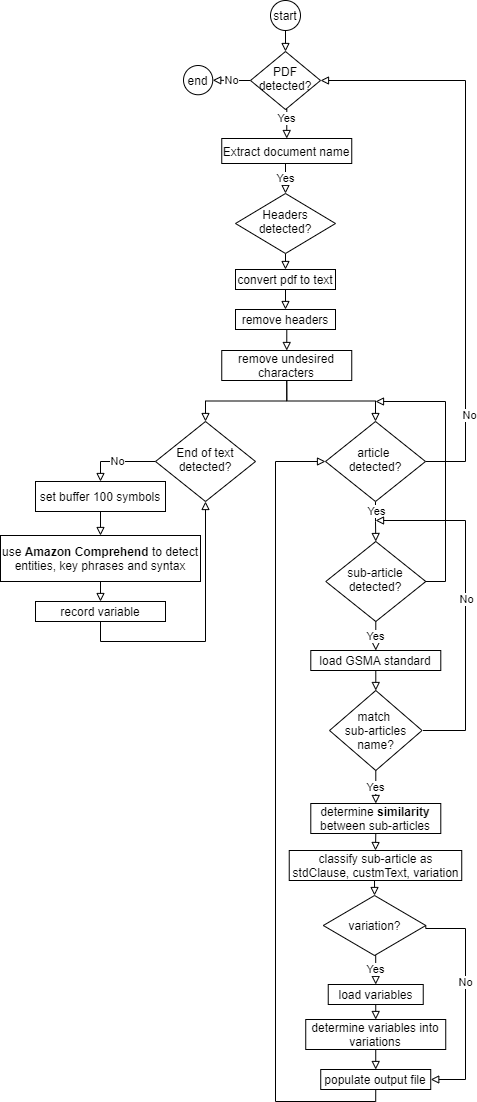
\includegraphics[width=0.4\textwidth]{images/methodology.png}}
\caption{Overview of the designed methodology.}
\label{fig1}
\end{figure}

The starting point of the methodology is the decompression and content extraction of PDF files (each PDF file contains a RA). The file name is used as one of the identifiers of the output file. The next step is to find similarities in document texts so that headers and footers are detected to avoid undesired characters. For that purpose, the mechanism used is the detection of different font sizes and weights. Once the PDF format has been converted to text is removed headers, and footers, as well as undesired characters (e.g., spaces, end-lines), in what is a parsing step. It is now possible to perform both \textit{detection} and \textit{comparison}.

The \textit{detection} phase includes a requirement associated with the Amazon Comprehend tool regarding the number of symbols to be sent via REST API. For this reason, the text is segmented into pieces of 100 symbols. For each symbol chunk the API outputs entities, key phrases and sentiment in JavaScript Object Notation (JSON) format~\cite{AWS2021}, which must be grouped and further processed. The designed logic collects the most important fields such as: 'BeginOffset', 'EndOffset', 'Score', 'Text', 'Type', 'PartOfSpeech', and 'Tag'. In turn, it adds to these the 'Frequency' field that indicates the number of repetitions of entities with same the same name, i.e., the same 'Text' field. Once this filtering has been done, entities are sorted according to a logic that defines their relevance degree. The designed logic is particularized according to the type of \textit{variable} to be detected. For instance, for the name of the MNO, the 'Score', 'Frequency', and 'BeginOffset' are prioritized, in addition to verifying the number of occurrences within the key phrases. The detected \textit{variables} are stored to be used later to determine which ones are part of the \textit{variations} or \textit{customized texts}.

The \textit{comparison} phase implies to separate by articles and then by sub-articles. Since several of the possibilities of article names are loading in the NLP Engine is easy to locate the corresponding article in the GSMA standard template and therefore, to establish comparisons at the sub-article level. \textit{Jaccard's similarity} associates a score to the sub-article ID. Thus, a sub-article is considered a \textit{standard clause} whether the score assigned is greater than 0.85 (score $\geq$ 0.85). In addition, a sub-article is considered a \textit{custom text} whether the score assigned is less than 0.15 (score $\leq$ 0.15). Finally, a sub-article is considered a \textit{variation} whether the score assigned is between 0.85 and 0.15 (0.15 $<$ score $<$ 0.85). At this point, the NLP Engine is ready to populate the output file, inspecting in case of to have tagged the sub-articles as \textit{variation} or \textit{customized texts}, the \textit{variables} that it contains.